\chapter{Experiments and Applications}

In the previous two chapters the mathematical and computational challenges of image reconstruction for CT have been discussed. In chapter 3, a detailed description of a variety of different algorithms has been presented, including the ART family of algorithms, CGLS, MLEM and few TV approaches for smooth reconstruction, as well as the classic FDK reconstruction. Additionally in chapter 4 the computational aspect of CT is discussed, on where the problems computing the exact adjoint of the projection operation and mainly the computational burden of some of the operations have been mentioned. Considering the variety of available methods and the specifics of the implementation of the software developed, the TIGRE toolbox, experiments on how these algorithms compare and behave are due. Further than that, the performance of these algorithm in different experimental datasets is also an important analysis.

This chapter shows experimental analysis on both of the topics. First a variety of convergence analysis with different algorithms using synthetic data are performed, showing the differences not only between algorithms, but also between option on parameter selections. The section tries to illustrate and perhaps help build intuition on all the different parameters and options that each of these algorithms has, both within the algorithms themselves and among the different ones. Additionally some highlights on the practical challenges that the use of the algorithms entail in real applications are given.

In the second section of this chapter, a few examples of some of the algorithms are shown in different CT applications, both cone and parallel beam. Data from various different applications, from medicine to science has been tested using the TIGRE toolbox. While quantitative analysis is not possible with these datasets because the truth is not known, some insight in how the algorithms behave in each case is discussed.

\section{Algorithm Experiments}
This section experiments with a variety of algorithms and parameter within then, and shows how they behave with different synthetic data in simulation studies. 

\subsection{Convergence rates}

On chapter 3 various times the convergence rates of the algorithms have been mentioned, as well as computational times. Different algorithms will reach to different residuals at the same iteration, and thus understanding which ones can converge faster, thus give a better result earlier, is important. However, at the scale of the CBCT problem, faster no only means reaching a residual that is smaller in the same iterations, as the computational burden of each of the iterations also needs to be considered. And, as the backprojection operator is not exactly the adjoint of the projection operator, an effect that the classic formulation of these algorithms do not take into account can happen: divergence. All the algorithms (at least in this work) are mathematically designed to always reduce the residual each iteration, but that formulation relies on a correct adjoint operator. Thus, sometimes, when the algorithms in TIGRE have a solution very close to minimum residual solution, they may diverge. The code in the toolbox does generally check for divergence and stop, but one of the effect that can be observed is that some algorithm will always diverge in a residual that is larger than others. This means that some algorithm can, regardless of their computational times, reach to a better solution than others.

All test in this section are performed in the XCAT phantom\cite{XCAT}, in a $128^3$ voxel size and $256^2$ detector. Different number of angles are used, always uniformly distributed along the full circle. Figure \ref{fig:XCAT} shows cross sections of the phantom on its middle plane and figure \ref{fig:XCATproj} shows 3 projections of the phantom as simulated for the following tests. 

\begin{figure}[h]
\begin{center}

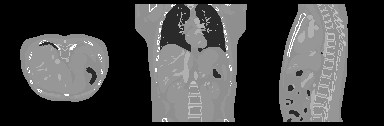
\includegraphics[width=0.9\textwidth]{Applications/XCAT.png} 
\end{center}

\caption[Cross section of the XCAT phantom]{\label{fig:XCAT} Cross section of the XCAT phantom in its middle plane in the three axis, for $128^3$ voxels.} 
\end{figure}

\begin{figure}[h]
\begin{center}

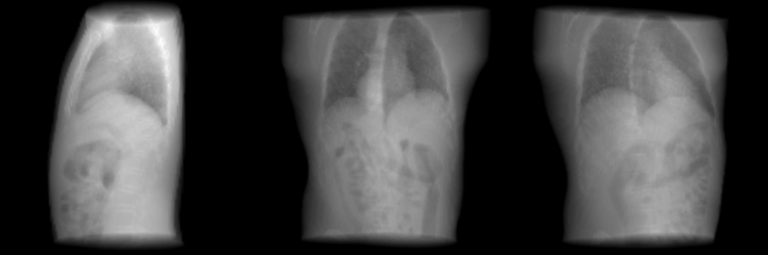
\includegraphics[width=0.9\textwidth]{Applications/XCATproj.png} 
\end{center}

\caption[Simulate projections of the XCAT phantom]{\label{fig:XCATproj} Simulate projections of the XCAT phantom in three different projection angles for a $256^2$ detector.} 
\end{figure}

\textbf{Update ordering in SART}. An analysis in the different ART-type algorithms is presented in this section first. One of the discussed parameters that has an effect in the convergence rate of the ART-type algorithms is the ordering of the used projections. Research has shown that in ART, the convergence rates with respect to how the rows are chosen for the updates is significantly changed[CITE], however in the algorithms feasible for big scale tomography, this effect is seen in a smaller scale. Figure \ref{fig:SARTanglesconv} shows the convergence of SART during 150 iterations using 50 projections as data. The same configuration of SART is run using ordered, randomly ordered and angular distance maximizing ordering schemes for the update order. While minor, the figure shows how random ordering does generally increases the convergence rate of the algorithm, at no computational cost. This is the default value in the software. Note that in this test there is no reduction of the relaxation parameter $\lambda$.


\begin{figure}[H]
\begin{center}

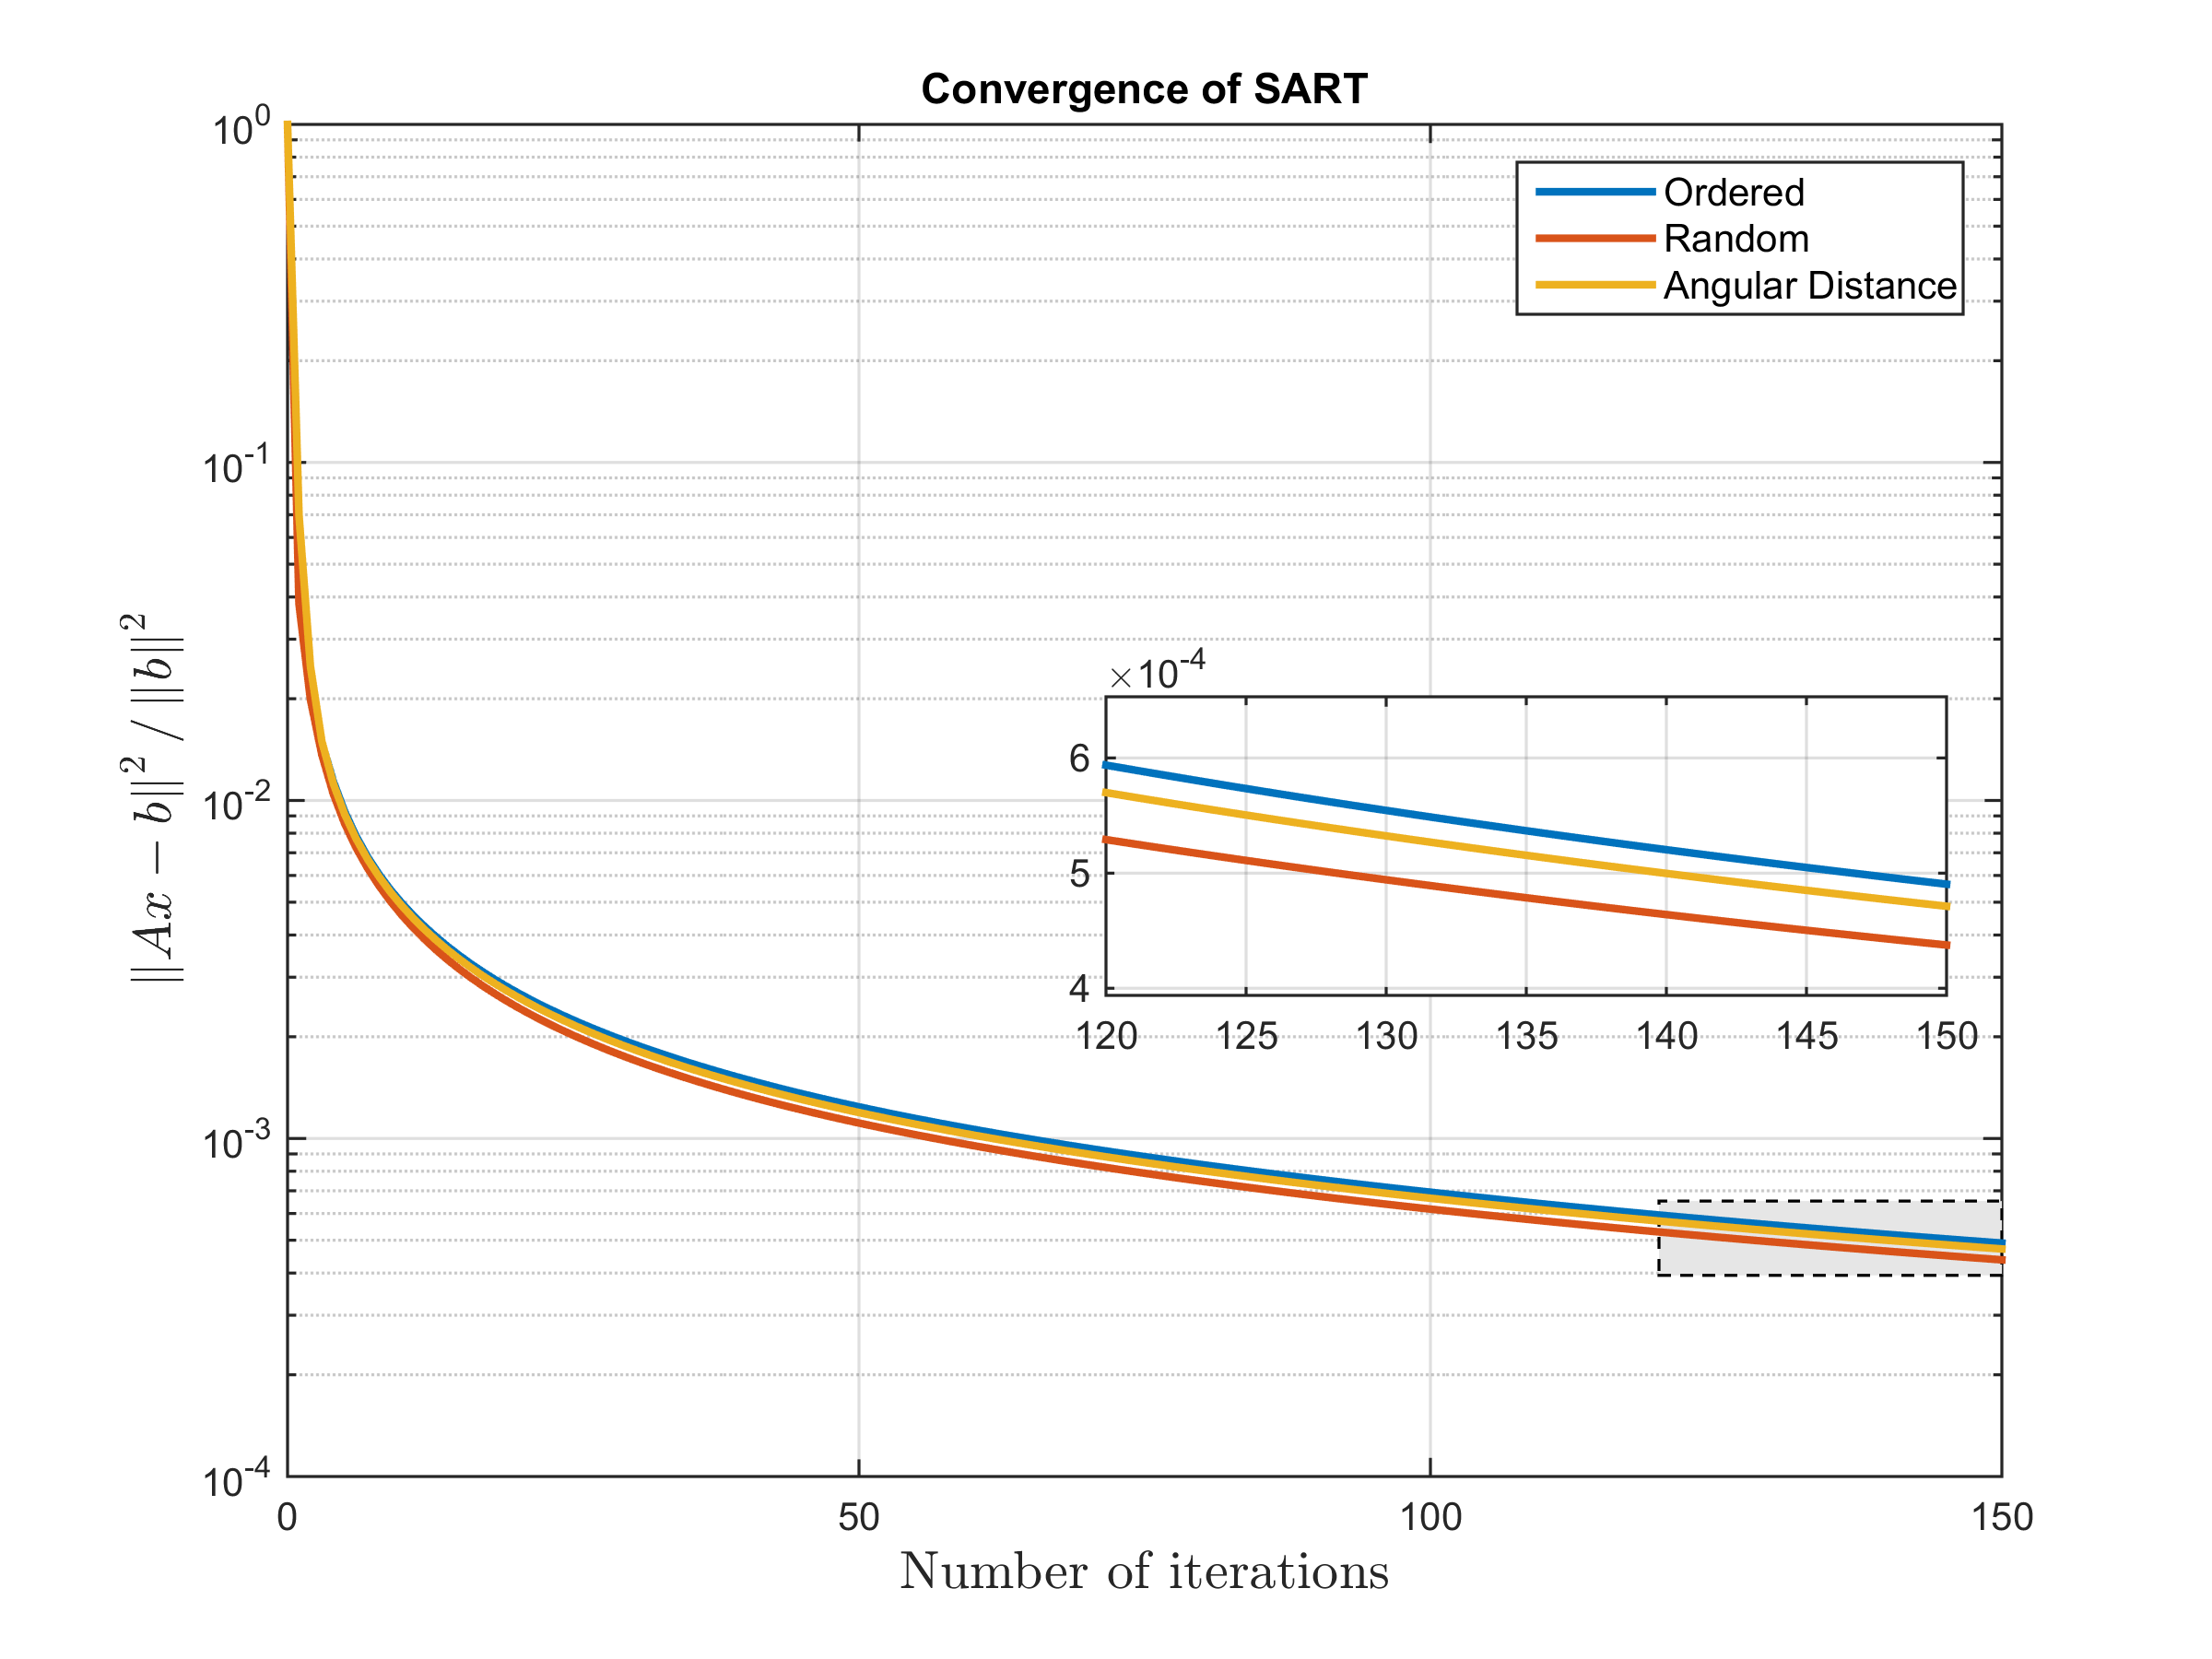
\includegraphics[width=0.8\textwidth]{Applications/SARTangles.png} 
\end{center}

\caption[Convergence of SART vs projection update order]{\label{fig:SARTanglesconv} Convergence of SART compared to different angle ordering schemes, using 50 projections and no relaxation parameter reduction} 
\end{figure}

\textbf{Comparison between SART, OS-SART and SIRT}. These algorithms have very different convergence, as updating the image per-equation has the effect of converging faster. However, the computational times are greatly reduced by updating more rows at the same time. This effect can be seen in figure \ref{fig:SARTtypesconv}, on where the convergence versus iteration of these three algorithms is plotted. Note the convergence difference between SART and SIRT, where SIRT doesn't reach SART's residual even after 1000 iterations, however, each iteration of SIRT is two orders of magnitude faster than SART. OS-SART provides a middle ground alternative. Due to the specifics of the acceleration procedures for backprojection, OS-SART speeds are closer to SIRT than to SART (i.e. the speed does not change linearly with the image updates per iteration), however it is more prone to divergent behaviour in TIGRE. In the figure, OS-SART stops converging after 48 iterations. Of course, this behaviour is very data-specific, and there are multiple cases where it does not diverge. Figure XX shows the result images of these three algorithms after 150 iterations (48 for OS-SART). Note that the example being show is low data, so even in the best case, the images are slightly noisy.



\begin{figure}[H]
\begin{center}

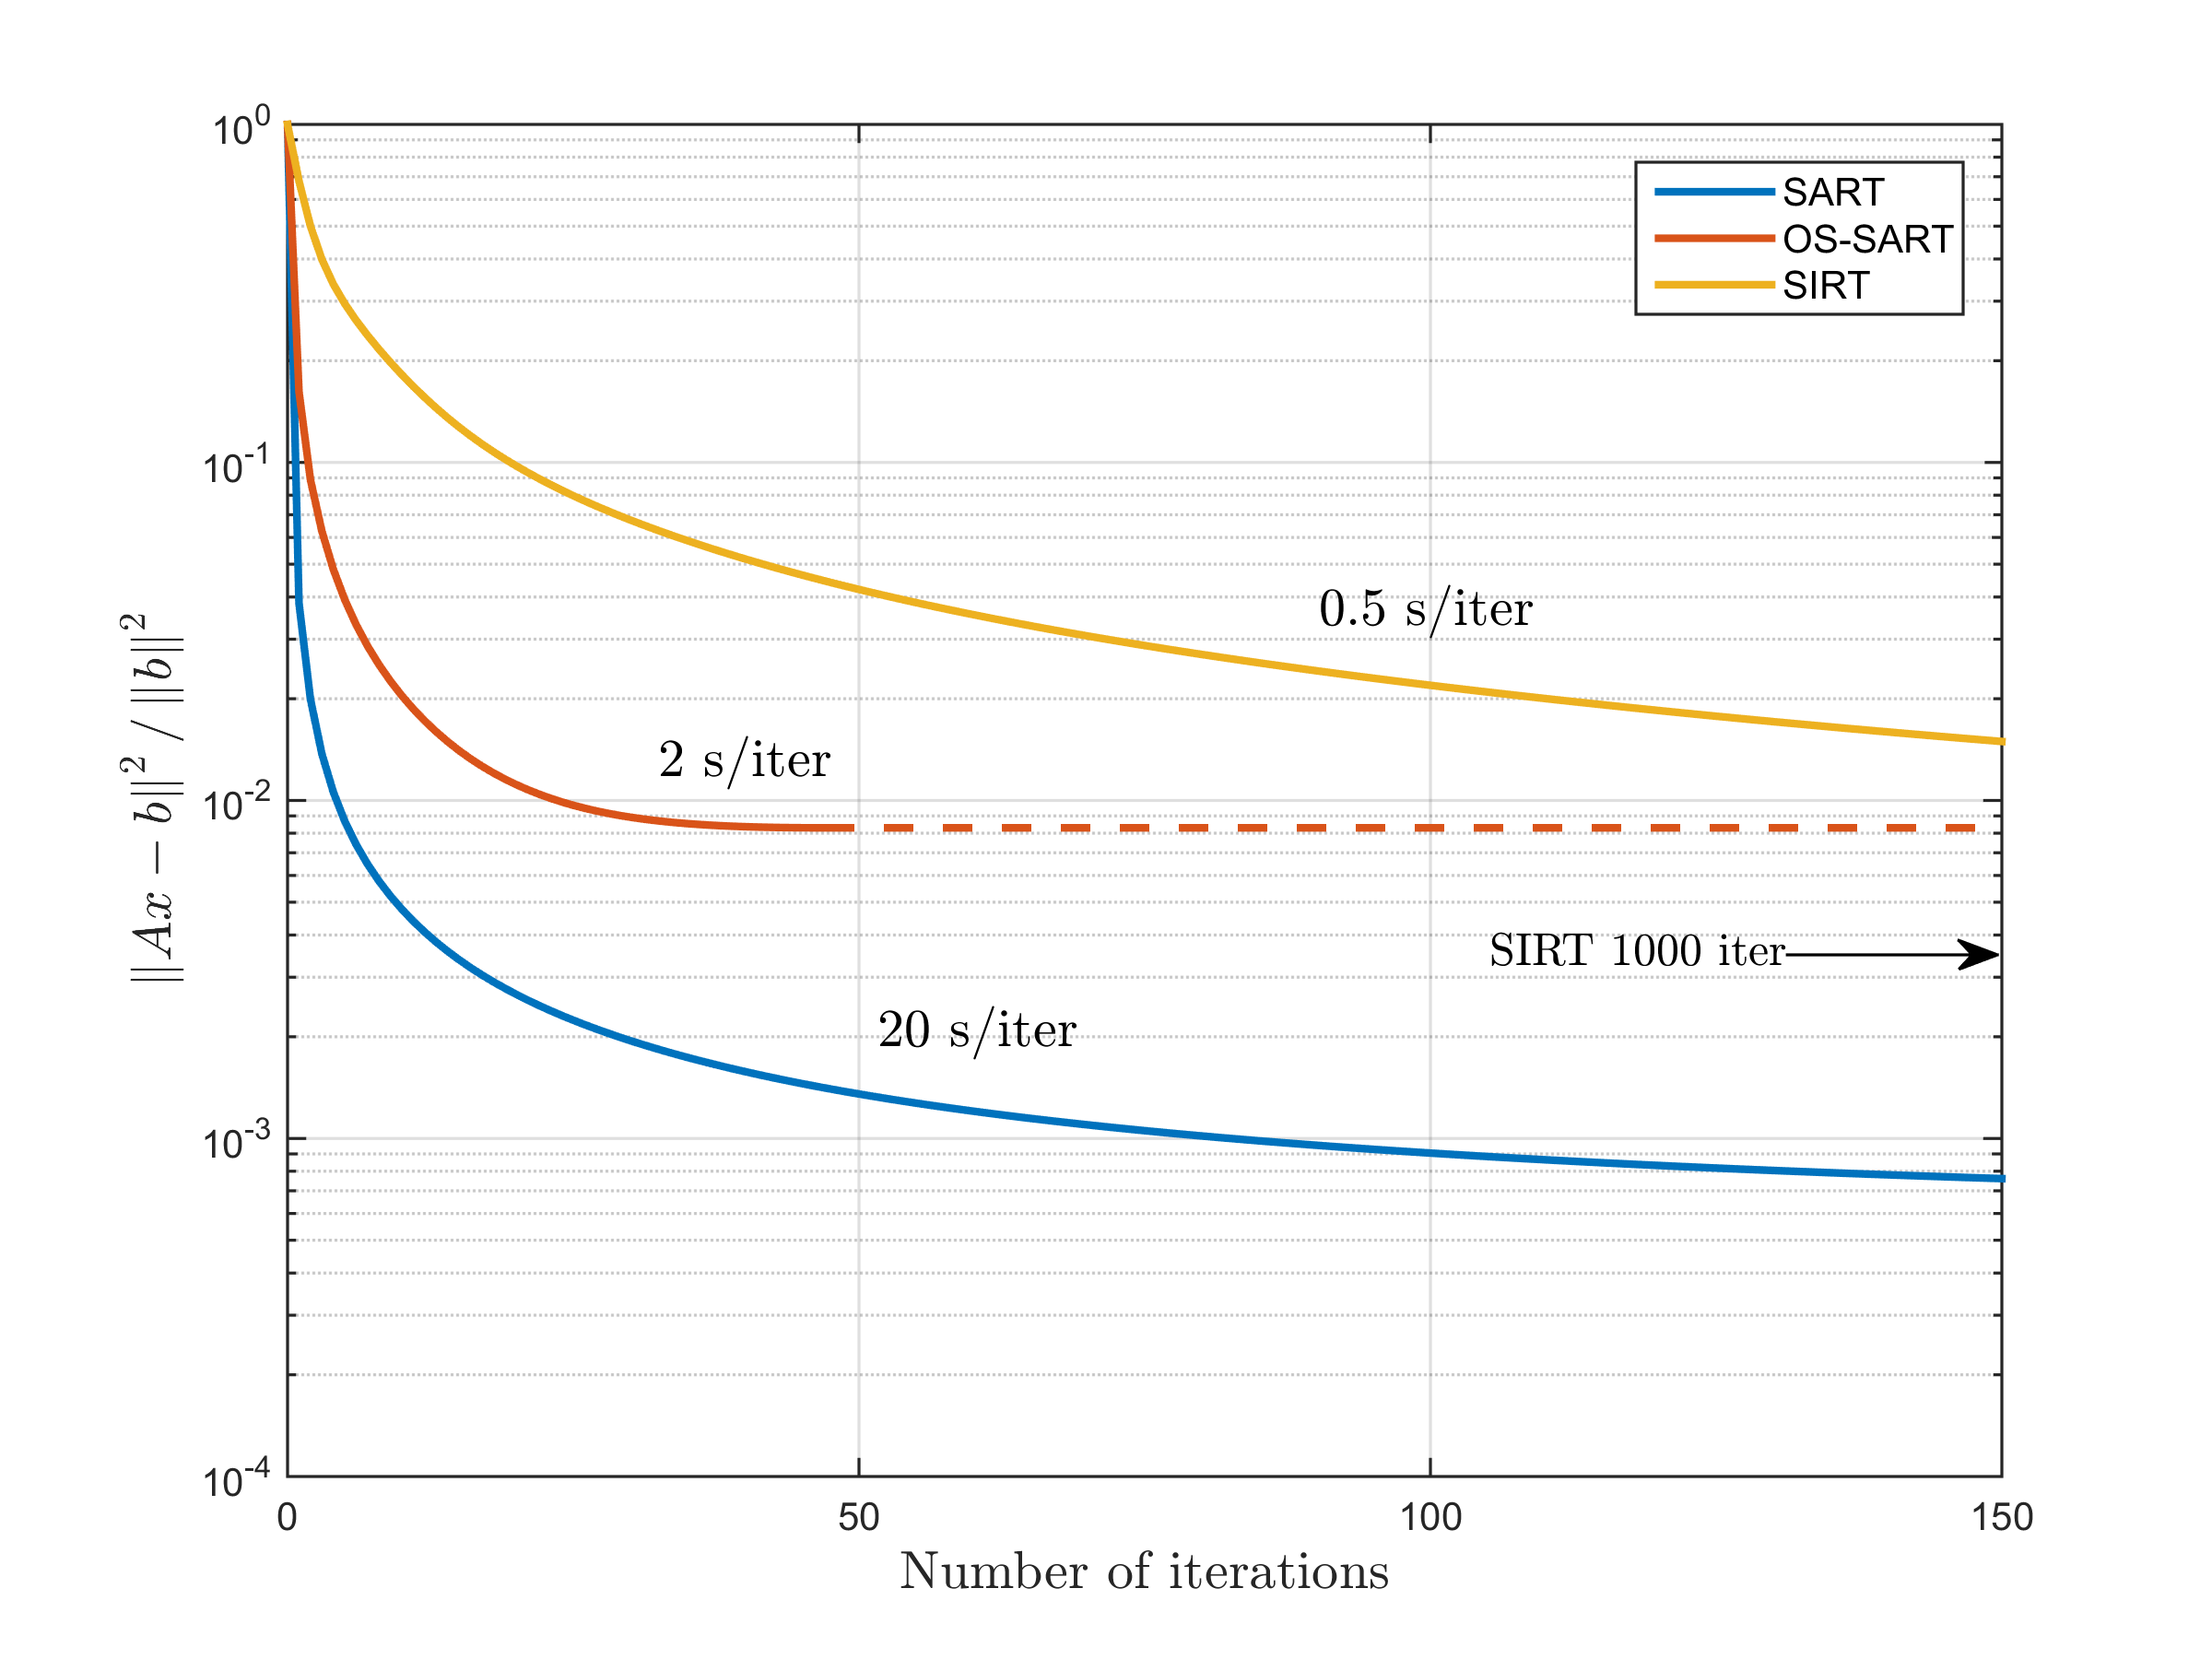
\includegraphics[width=0.8\textwidth]{Applications/SARTtypes.png} 
\end{center}

\caption[Convergence of SART/OS-SART/SIRT]{\label{fig:SARTtypesconv} Convergence of SART, OS-SART and SIRT using 50 projections and no relaxation parameter reduction.} 
\end{figure}



\subsection{Total variation minimization}


\section{Iterative Algorithms in Different CT Applications}
\subsection{Medical Head CBCT from  The Christie Hospital}
\subsection{Cryo Soft X-Ray Tomography at Diamond Light Source}